\subsection{Kuroda Transformation}

Die   Umwandlung   von   LC-Filter   in   Leitungsfilter    ist    dank    der
Richards-Transformation recht einfach, jedoch  wird  man  bei der Realisierung
als Mikrostreifenfilter auf Probleme stossen.

\begin{figure}[h!]
    \centering
    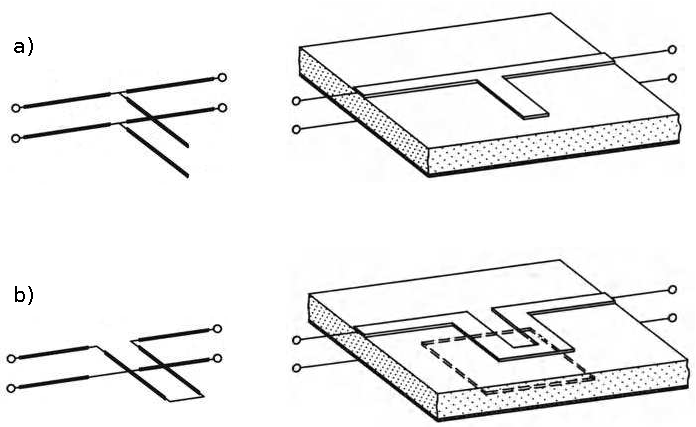
\includegraphics[width=\imagewidth]{images/mikrostreifen}
    \caption{Auszug aus dem Buch Mikrowellentechnik\cite[p.~27]{ref:baechold}: Realisierung von Stichleitungen in Mikrostreifentechnik: a: leerlaufende, geerdete Leitung und b: kurzgeschlossene, erdfreie Leitung}
    \label{fig:mikrostreifen}
\end{figure}

Gem\"ass  Figur   \ref{fig:mikrostreifen}a  kann  die  leerlaufende,  geerdete
Stichleitung  als  Einzelleitung  recht  gut  in  Mikrostreifentechnik  gebaut
werden. Nach  Figur \ref{fig:LC-zu-Leitungsfilter} sollten die Leitungen 1 und
3  am  Fusspunkt  der  kurzgeschlossenen  Stichleitung  2,  also  mit  kleinem
gegenseitigem  Abstand,  angeschlossen  werden. Da eine gegenseitige  Kopplung
zwischen  1 und 3 unerw\"unscht  ist,  f\"uhrt  diese  enge  Nachbarschaft  zu
Problemen.  Die  kurzgeschlossene  Stichleitung  2  l\"asst  sich,  wie  Figur
\ref{fig:mikrostreifen}b zeigt,  nur  schlecht realisieren. Die Induktivit\"at
sollte  in Form einer erdfreien,  kurzgeschlossenen  Stichleitung  erscheinen.
Eine elektrisch und geometrisch wenig befriedigen-  de  Anordnung ist in Figur
\ref{fig:mikrostreifen}b gezeigt, wo mit einer  \"Offnung  in  der Grundplatte
eine  gewisse  Erdfreiheit  erzielt  wird.  Dieses  Beispiel  zeigt,  dass die
vorliegende    Tiefpassstruktur    nicht   f\"ur    eine    Realisierung    in
Mikrostreifentechnik   geeignet  ist.  Es  w\"are  von   Vorteil,   wenn   nur
kurzgeschlossene oder leerlaufende  Stichleitungen  gegen die Grundplatte (mit
einer  Leiterseite an Erde) auftreten w\"urden.  Weiter  w\"are  eine  gewisse
Distanz  zwischen  den  Leitungselementen   vorteilhaft,   um   unerw\"unschte
Kopplungen  zu  vermeiden.  Genau  diese Anspr\"uche werden weitgehend mit der
Kuroda-Transformation    befriedigt,    wie    nachfolgend    gezeigt    wird.

Neben den kurzgeschlossenen und leerlaufenden Stichleitungen f\"uhren wir  als
zus\"atzliches  Leitungselement  das  Einheitselement (unit element) U.E. ein,
welches ein St\"uck \"Ubertragungsleitung mit einer Wellenimpedanz Zue und der
gleichen L\"ange I wie die Stichleitungen darstellt.

\begin{figure}[h!]
    \centering
    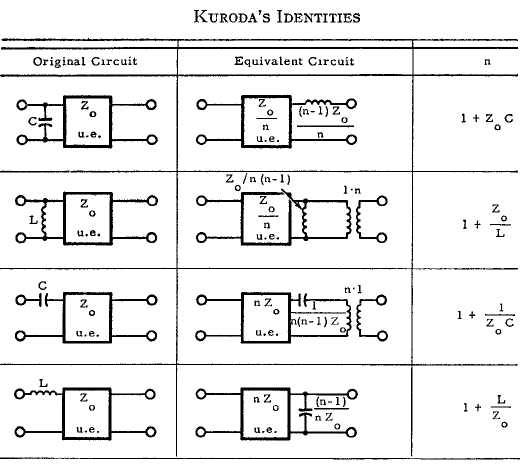
\includegraphics[width=\imagewidth]{images/kuroda-identities}
    \caption{Kuroda-Identit\"aten}
    \label{fig:kuroda-identities}
\end{figure}

